\chapter{Проектиране на печатните платки}

За проектирането на печатните платки и монтажните схеми в проекта е използван софтуерния пакет KiCad. Той е избран за целта, защото е безплатен и има богата библиотека с компоненти, съдържащи символи и \textbf{??} очертания на корпуси \textbf{??}.

%================================================================================
% ЕЛЕКТРИЧЕСКА СХЕМА  -  РОБОТ

\section{Принципна електрическа схема на робота}

Принципната електрическа схема на печатната платка в робота може да бъде видяна на \textbf{??} приложение \textbf{??}. Основният елемент на схемата е микроконтролерът STM32F103C8T6 (blue pill), който управлява останалите компоненти. Използваните компоненти в проектирането на тази печатната платка могат да бъдат видяни в таблица \textbf{????} приложение \textbf{????}



\subsection{Радиочестотен модул}

Връзката между дистанционното и робота се осъществява посредством nRF24L01+ PA/LNA радиочестотен модул. Комуникацията между него и използвания микроконтролер е посредством SPI интерфейс. Радиочестотният модул бива захранван с 3,3V от вградения регулатор на напрежението на blue pill. С цел повишаване на съотношението сигнал/шум са поставени 100nF керамичен кондензатор и 100uF електролитен кондензатор, които да намалят съответно високочестотните и нискочестотните шумове.

предавател по далеч / мощни мотори = повече шум
слаб сигнал

+ какво е ПА/ЛНА 
+ режим на СПИ интерфей и неговата скорост
\begin{figure}[H]
    \centering
    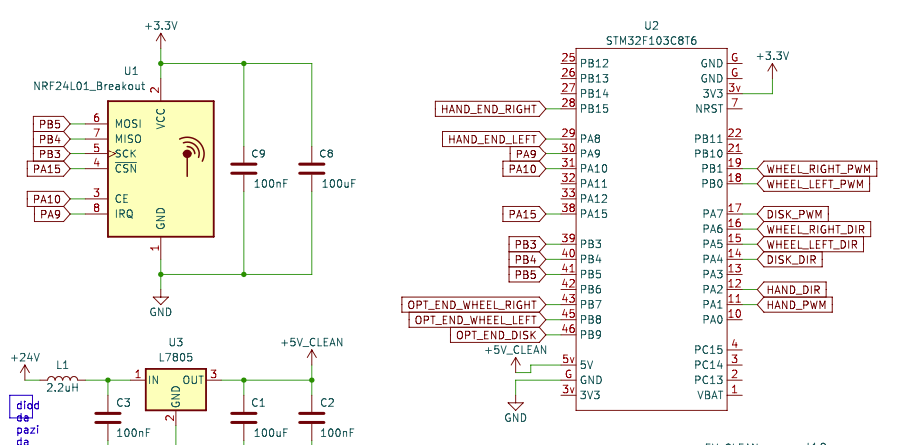
\includegraphics[width=0.6\linewidth]{images/rf-module.png}
    
    \caption{Радиочестотен модул}
    \label{fig:rf-module} 
\end{figure}



\subsection{Управление на моторите}

Управлението на постоянно токовите четкови мотори се извършва посредством MD13S драйвери. Необходимите логически сигнали за да може да се реализира управлението са ШИМ сиганл, който упоменава скоростта, с която мотора трябва да се върти, и високо или ниско ниво, което да показва посоката на движение
\textbf{????}\footnote{Ужасно изказано}.
С цел изолация между микроконтролера и драйверите са поставени оптрони. Начинът на свързване на всеки оптрон може да бъде видян на \cref{fig:brushed-control}. Необходимото захранване на всеки мотор е 24V и то бива подадено посредством отделен конектор.


\begin{figure}[H]
    \centering
    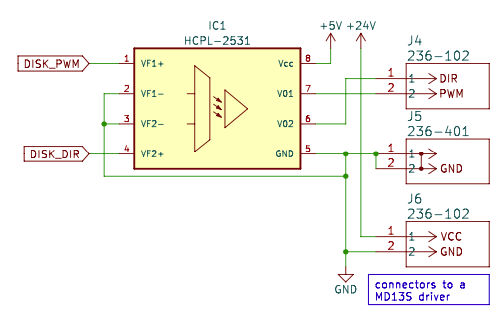
\includegraphics[width=0.6\linewidth]{images/brushed-control.png}
    
    \caption{Оптрон}
    \label{fig:brushed-control} 
\end{figure}


За управлението на стъпковия мотор се използва драйвер DM556T. Сигналите за управление включват ШИМ сигнал, който определя стъпките за изпълнение и логическо ниво (високо или ниско), указващо посоката на движение \textbf{????}\footnote{Ужасно изказано}.
Не е поставен допълнителен оптрон за изолация между драйвера и микроконтролера, поради причината, че на входовете си DM556T има вградени такива. Така направена схемата обаче няма да работи, защото логита на blue pill-а е на 3,3V, докато драйвера използва 5V логика. Този проблем бива решен като се използва преобразувател на логически нива U12, който превежда логическото управление от 3,3V към 5V, съответстващо на логиката, използвана от драйвера.

\begin{figure}[H]
    \centering
    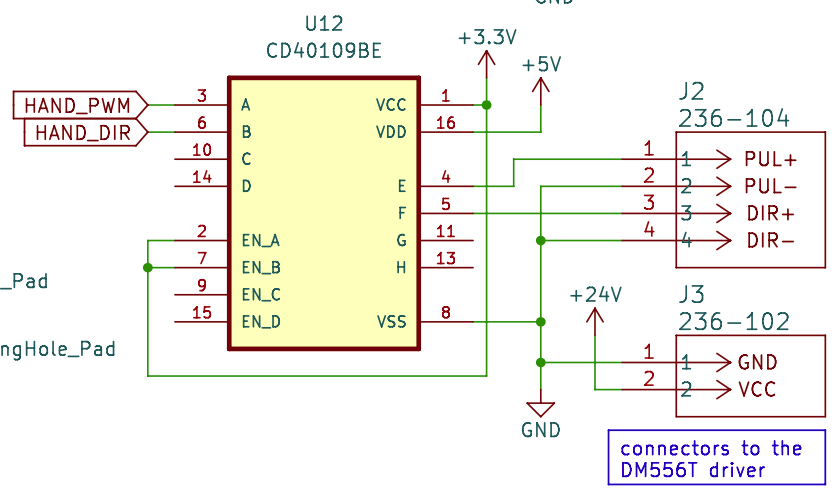
\includegraphics[width=0.6\linewidth]{images/stepper-control.png}
    
    \caption{Левел шифтър}
    \label{fig:stepper-control} 
\end{figure}



\subsection{Сензори}

За следене на скоростта на робота са предвидени и инсталирани оптични сензори. Те биват свързвани към печатната плака чрез конекторите J10, J11 и J12. Всеки сензор има извод за данни и изводи за захранване. 

\begin{figure}[H]
    \centering
    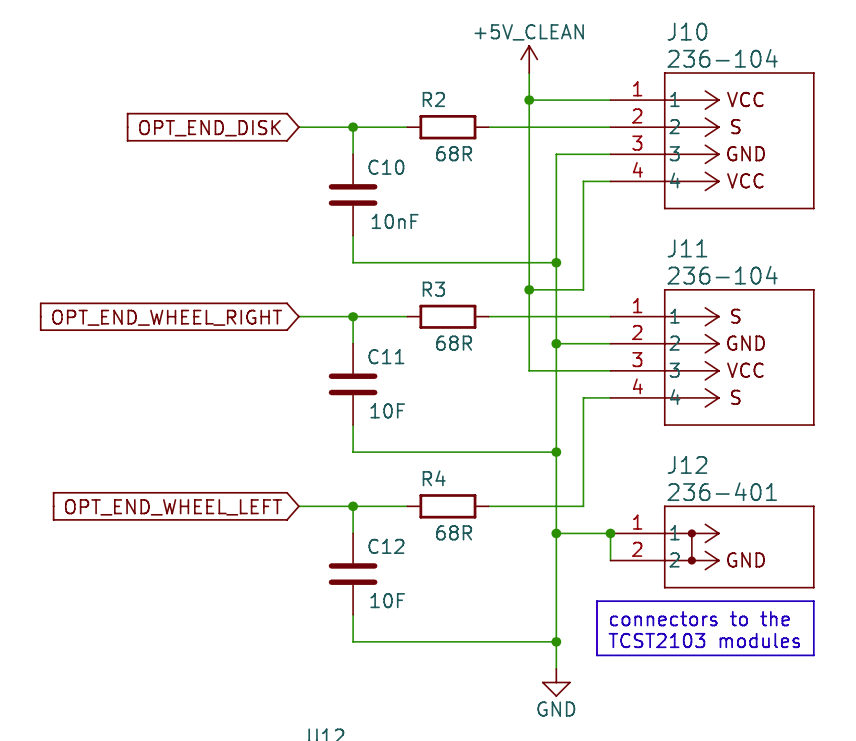
\includegraphics[width=0.6\linewidth]{images/optical-sensors.png}
    
    \caption{оптични сензори}
    \label{fig:optical-sensors} 
\end{figure}

Съгласно изискванията за безопасност са предвидени и крайни изключватели, които да следят дали стъпковият мотор е достигнал някоя от крайните си позиции. Те са свързани, чрез конекторите

\begin{figure}[H]
    \centering
    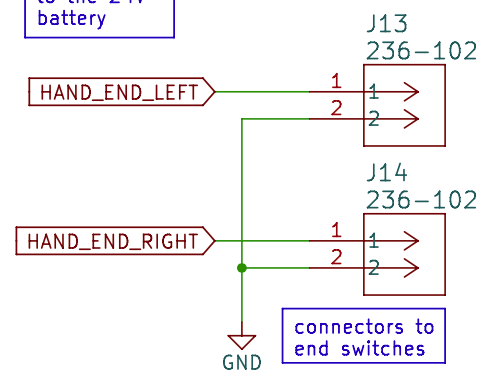
\includegraphics[width=0.6\linewidth]{images/hand-endswitches.png}
    
    \caption{Крайни изключватели за ръката}
    \label{fig:hand-endswitches} 
\end{figure}


\subsection{Захранване на печатната платка}

Печатната платка се захранва директно от 24V постояннотокова батерия. Съгласно изискванията за безопасност изводите на конектор J15 са предвидени за ключ, който да спира цялото захранване на робота. Освен това има имплементирани хардуерни защити против късо съединение, пренапрежение и обратен поляритет на захранването. Първата от трите е реализирана чрез поставянето на автомобилен бушон на държача X1 последователно свързан след главния ключ. Защитата против пренапрежение се осъществява посредством двупосочния трансил D3, който има номинално напрежение \textbf{????}. С цел застраховка против неправилен поляритет на напрежението е поставена P-MOS защита след трансила. Тя се реализира чрез транзистора Q2, ценеровия диод D1 и резистора R1. При правилното свързване на батерията през диода в Q1 протича ток. Поради образувания делител на напрежение D1 и R1, напрежението гейт-сорс на Q2 става равно на пробивното напрежение на D1 и транзисторът се отпушва. В случай, че батерията бъде свързана с обратен поляритет, диодът в Q1 бива свързан в обратна посока и транзисторът остава запушен. 
\textbf{????}\footnote{Стабилизиране на напрежението чрез кондензатора C7}

\begin{figure}[H]
    \centering
    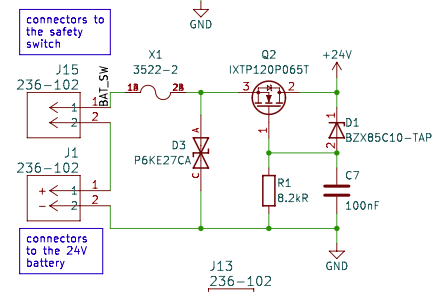
\includegraphics[width=0.6\linewidth]{images/power-protection.png}
    
    \caption{Защити на захранването}
    \label{fig:power-protection} 
\end{figure}

Захранването на логическата част на проекта е постигнато посредством линейни стабилизатори L7805. Tо е разделено на два канала за да може да бъдат намалени шумовете в захранването на микроконтролера и радиочестотния модул \textbf{????}\footnote{Да кажа от къде идват шумовете}. 

Първият канал използва стабилизатора U4 за да успее да свали напрежението до 5V, които да бъдат подадени после на оптроните на логическата част на четковите мотори и на логическия преобразовател на стъпковия мотор. Той е показан на \cref{fig:power-5V}. За намаляване на шумовете в системата са поставени нискочестотния филтър C5 и високочестотния филтър C6. \textbf{????}\footnote{За допълнително стабилизиране на захранването е добавен кондензатора C4 - функция}. 

Вторият канал на захранването е почти идентичен с първия. Той се използва за захранването на микроконтролера, радиочестотния модул и сензорите в робота и може да бъде видян на \cref{fig:power-5V-clean}. \textbf{????}\footnote{бобината L1}.
+две захранвания не два канала
\begin{figure}[H] 
    \centering
    \begin{subfigure}[h]{0.6\textwidth}
        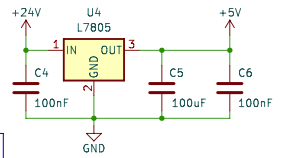
\includegraphics[width=\textwidth]{images/power-5V.png}
        \caption{Захранване на логиката на силовата електроника}
        \label{fig:power-5V}
    \end{subfigure}
    \\ %add desired spacing between images, e. g. ~, \quad, \qquad, \hfill etc. 
      %(or a blank line to force the subfigure onto a new line)
    \begin{subfigure}[h]{0.75\textwidth}
        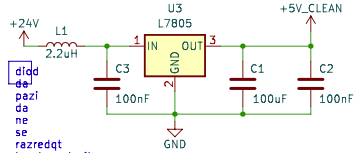
\includegraphics[width=\textwidth]{images/power-5V-clean.png}
        \caption{Захранване на микроконтролера, радиочестотния модул и сензорите}
        \label{fig:power-5V-clean}
    \end{subfigure}
    ~ %add desired spacing between images, e. g. ~, \quad, \qquad, \hfill etc. 
    %(or a blank line to force the subfigure onto a new line)    
    \caption{Захранване на логическата част в робота.}
    \label{fig:power-low}
\end{figure}

%================================================================================
% PCB layout  -  РОБОТ

\section{Опроводяване на печатната платка на робота}

%================================================================================
% МОНТАЖНА СХЕМА  -  РОБОТ

\section{Монтажна схема на робота}

Монтажната схема на робота може да бъде намерена в \textbf{??} приложение \textbf{??}. На нея може да се види основната част в робота, представляваща разработената печатна платка, която съдържа радиочестотния модул за комуникация, микроконтролера, управляващ робота, и хардуерните защити на захранването. Нейното захранване индва от 24V батерия DeWalt DE0241 и съгласно изисканията за безопасност във всеки момент то може да бъде прекъснато чрез ключът SW1. Разработената платка захранва и управлява 3 постояннотокови четкови мотори с помощта на драйвери MD13S. С цел мониторинг на тяхната скорост е предвидено на всеки от тях да има монтиран по един оптичен сензор за скорост. Използваният nema 24 стъпков мотор се управлява посредством DM556T драйвер. Начинат на свързване на драйвера към печатната платка е конфигурация общ катод. Съгласно изискванията за безопасност чрез SW1 и SW2 се следи дали стъпковият мотор не е стигнал до крайните си състояния.

+ параметри на входовете на драйверите

%================================================================================
% ЕЛЕКТРИЧЕСКА СХЕМА  -  ДИСТАНЦИОННО

\section{Принципна електрическа схема на дистанционното}

Принципната електрическа схема на печатната платка на дистанционното може да бъде видяна на \textbf{??} приложение \textbf{??}. Основният елемент на схемата е микроконтролерът STM32F103C8T6 (blue pill), който чете данните от сензорите, обработва ги и после ги праща към робота посредством радиочестотния модул. Използваните компоненти в проектирането на тази печатната платка могат да бъдат видяни в таблица \textbf{????} приложение \textbf{????}



\subsection{Радиочестотен модул}

\subsection{Сензори}

%================================================================================
% PCB layout  -  ДИСТАНЦИОННО

\section{Опроводяване на печатната платка на дистанционното}

%================================================================================
% МОНТАЖНА СХЕМА  -  ДИСТАНЦИОННО

\section{Монтажна схема на дистанционното}

\textbf{????}\footnote{Трябва ли да има такова нещо изобщо}